\documentclass[0main.tex]{subfiles}

\graphicspath{{./img}}
\begin{document}
\section{Intelligent Transport Systems}\label{sec-its}

This section focuses on examining various existing ITS solutions and attempting to recognize their
agent-based characteristics and principles in order to determine the possible application of MAS for
simulation of ITS systems.

Intelligent transport systems describe an initiative to utilize modern technology 
to optimize and increase the efficiency of processes common to the domain of transportation. 
This usually involves enabling different actors in the transportation system to communicate 
with each other and share available information (much like multi-agent systems). With the 
availability of shared information, complex, data-driven systems can be built utilizing 
state-of-the-art technology like machine learning, computer vision and IoT. Integrating 
such concepts with road users to improves traffic safety and increases traffic efficiency.
It also addresses environmental issues by controlling traffic to prevent congestion or lessen
their adverse effects. 

Looking these solutions from a systemic point of view, they can, more or less, resemble
multi-agent systems. Such approach answers whether a suitable application for agent-based
modeling of ITS is feasible. The insights gained by reviewing the current state of ITS will
serve as a base for further sections, where considerations regarding framework design and
its validation are discussed. 

ITS provides itself most useful in the following aspects of transportation: \emph{Mobility},
\emph{Safety}, \emph{Environment} \cite{Lishchenko2021}. To provide an example, regarding
mobility, one of the most common systems is routing and navigation for road users. These
systems can factor in time, distance and even emissions when providing route guidance
\cite{Firmin2006}. This leads to increased performance of road networks. Regarding safety, one
can mention emergency management systems like E-Call, which provides automated post-crash
assistance by contacting emergency services as soon as an accident occurs. In terms of the
environment protection, ITS allows for demand management through \emph{electronic fee
collection}, which makes flexible charging for road usage possible, based on vehicle type and
emissions category \cite{Commision2022}. Another, more general example of emissions reduction
of ITS is through reducing congestion, as road vehicle emissions are proven to pose a significant
negative factor for the environment. Especially because they produce emissions in
densely-populated areas, exposing a large population to serious health risks. In a study
conducted by the Harvard School of Public Health, air pollution from traffic congestion in 83
of the USA's largest urban areas contribute to more than 2,200 premature deaths annually,
costing the healthcare system at least \$18 billion \cite{Levy2011}.

\subsection{Simulator-based research}

Using virtual simulation tools to research and evaluate the impacts of ITS solutions 
greatly reduces the overall cost of product development. It also offers for fast-paced 
and flexible testing in virtual space allowing for frequent, iterative evaluation of features.

It is important to say that ITS solutions vary in terms of \emph{driver engagement}. Because
the primary use case of an IVS is to research driver behavior, the scope of the current state
of ITS is focused on ITS solutions that both integrate automotive transport and offer some
degree of driver engagement. 

To give an example, some ITS use cases with high driver engagement are listed \cite{Lishchenko2021}:

\begin{itemize}
    \itemspacing{.7}
    \item Geo-info service
    \item Real-time road condition service 
    \item Accurate traffic-info service 
    \item Real-time vehicle info service 
    \item Parking guidance service
\end{itemize}

These use cases shall be considered when modeling the ITS simulation framework in the practical part of the 
thesis.

\subsection{Intelligence distribution} \label{mas-compatibility}

It is important to acknowledge whether the underlying system control is centrally governed 
or whether the intelligence is distributed across multiple actors, where individual 
components of the system can act semi- or fully independently.
Such phenomena are important to consider because ITS solutions 
with centralized or distributed intelligence can be fundamentally different.
This leads to different system models being optimal to use when simulating a particular ITS. 
Intelligent transport systems are, by nature, systems combining several actors to
achieve a common goal. This, however, doesn't mean that it is optimal to model \emph{every} ITS 
as a multi-agent system. 

Historically speaking, ITSs that proved helpful for optimizing traffic were \emph{centralized}
\cite{Corman2010}, meaning there is a single, central component in charge of the
decision-making logic. A centralized traffic system organizes other units/actors within the
system, while interacting with the drivers in the traffic as external actors. The main
advantage of this approach is that is is less complex, therefore it is easier to develop a
resilient and safe product. The main drawback of this method is that it is heavily affected by
the size of instances, increasing the complexity and often resulting in exceedingly large
computation time, making the solution sub-optimal \cite{Corman2010}. 

As with the \emph{distributed} systems, the logic how to solve the main problem is systematically distributed to
individual agents solving a sub-problem and cooperating to achieve optimal and predictable
results. Such distributed intelligence is often modeled using \emph{Multi-agent Systems}. This
topic is further discussed in the section \ref{sec-mas}. Distributed systems can be used to
solve traffic optimization problems on a larger scale. These systems have seen larger usage,
especially in recent times, as newly produced vehicles come equipped with powerful computers.
This is leveraged to spread out the computational burden from the core computational unit in centralized
systems. A practical example of distributed intelligence solutions are the state-of-art
communication protocols like DSRC and ITS-G5, which enable low-latency direct communication
between vehicles. 

One example of ITS where implementations have been carried out in both centralized and 
decentralized principles numerous times is a \emph{Network traffic control}. The goal of this 
system is to use knowledge about the traffic on the network to control traffic lights and other 
active control elements to optimize traffic flow and decrease travel time. In a recent research 
that reviews signal timing optimization approaches compared centralized and distributed network traffic
control systems. The final conclusion is that although the centralized system is able
to achieve better performance and higher global efficiency, the decentralized solution requires
significantly less computation time (40 \% in their experiment case) \cite{Chow2019}.

Other decentralized systems that are more exposed to the user (i.e. driver) include the 
\emph{Adaptive Cruise Control} (ACC). ACC extends the usual cruise control systems 
that maintain vehicle speed by adapting to the speed of the vehicle in front.  
Recent development has led to further improvement, making ACC a cooperative system (CACC) that 
enables vehicles to adopt a \emph{driving strategy} by communicating with the infrastructure (V2I 
communication).

\subsubsection{Current research}\label{sec-research}

In general, it is important to examine systems that are time-relevant and bring benefit to
current as well as future IVS and Human-Machine Interface (HMI) research activities. Therefore,
this sub-section focuses on reviewing ITSs that are an ongoing subject to research and
current trends in the ITS industry, exploring state-of-the-art ITS solutions. To determine which ITSs
are relevant, ongoing projects of governmental bodies and their
strategies as well as the current trends in automotive ITS are reviewed.

In Europe, there are initiatives to centralize decision-making and ITS deployment on the scale of 
the European continent. The reason behind this initiative is quite clear - to enable Europe-wide 
interoperability between deployed ITS and ITS-enabled vehicles. 
Such organization would closely work with the industry, helping to create conditions for
deployment of novel ITS technologies.

\paragraph{ERTICO}

One such European organization is the \emph{European Road Transport Telematics
Implementation Coordination (ERTICO)} - a public-private partnership organization
with close to 120~members, connecting 8 different sectors in the ITS Community, including
service providers, suppliers, traffic and transport industry, research institutions and
universities, public authorities, user organizations, the connectivity industry as well as
vehicle manufacturers \cite{ertico}.

As of now, ERTICO's activities focus on the following areas:

\term{Connected Cooperative \& Automated Mobility}
The computational power of newly-produced vehicles is increasing dramatically with every 
new generation, as well as the number of sensor data. ERTICO states that their focus is on utilizing 
the large amounts of real-life data to deepen the machine learning models, as well as building 
infrastructure that will allow handling this data. C-ITS (Cooperative Intelligent Transport
Systems) is also a topic that ERTICO is invested in. C-ITS is being put into practice by several projects, 
namely European Truck Platooning (ETPC), Advanced map-enhanced driver assistance systems (ADASIS) and 
more. ERTICO's main contribution is to facilitate the creation of the ITS ecosystem by following a
multidisciplinary approach involving all relevant transport stakeholder sectors.

\term{Clean \& Eco Mobility}
As has been already mentioned, smart mobility innovations make a major contribution towards 
reducing the impact of transport-induced pollution, which has got a non-negligible contribution to 
global greenhouse gas emissions production \cite{Ritchie2020}. Below are the four main
objectives in the area of Clean \& Eco-Mobility \cite{ertico}.

\begin{itemize}
    \setlength\itemsep{-10pt}
    \item Develop a common approach to the evaluation of ITS deployment as a tool for emissions reduction
    \item Contribute to smart mobility solutions being recognized as a tool for reducing emissions
    \item Achieve interoperability of electro-mobility
    \item Contribute to creating an ICT network with seamless and interoperable electro-mobility services
\end{itemize}

\term{Urban Mobility}
Another focus of ERTICO is Urban Mobility, where the main goal is to provide "Mobility as a Service" (MaaS), 
which is a system that could decrease congestion and provide low-carbon and -emission multi-modal transport 
solutions.  

\term{Transport \& Logistics}
ERTICO states that the current European world of transport and logistics is too fragmented, so an effort to 
developing a solution for connecting logistics information systems would optimize cargo flows and facilitate supply 
chain management. 

In conclusion, the ERTICO organization helps to reduce the time to market of innovative,
state-of-the-art technologies, increasing inter-operability between individual ITS by promoting
an open framework for the integration and deployment of intelligent transport services. 

As described above, there are potential systems that are yet to be fully implemented and
deployed for consumer use. 

\paragraph{Cooperative ITS}

Cooperative Intelligent Transport Systems (C-ITS) refer to transport systems where ITS 
subsystems (personal, vehicle, roadside and central) cooperate. This
enables and provides an ITS service that offers better quality and an enhanced service level,
compared to the same ITS service provided by only one of the ITS sub-systems \cite{2022}.

The concept of C-ITS was developed by the European Commission, representatives of industry and 
authorities in the European Union. In 2016, the bodies agreed on a coordinated establishment of intelligent
transport systems in Europe. It is considered to be one of the tools to facilitate achieving 
the \emph{vision zero}, which is a project that aims to mitigate all fatalities involving road 
transport.

The European Commission outlined its plan for the coordinated deployment of C-ITS in Europe in
its communication "A European strategy on Cooperative Intelligent Transport Systems", in which
it also states that the full-scale deployment of C-ITS services and C-ITS-enabled vehicles were
expected to start in 2019.

The main feature of C-ITS is its distributed intelligence across vehicles and the infrastructure, 
which is a novel concept in the ITS world. Consequently, it is easy to see similarities in how a
MAS is described. Regarding the topic of this thesis, this could pose an argument to
implement one of the C-ITS systems in the practical part of this thesis.

Vehicles and infrastructure equipped with C-ITS can, for example, communicate a traffic-related warning to each
other. Upon receiving such warning, the drivers are informed about the upcoming traffic situation in time for
them to take the necessary actions to avoid potential harm. Other potential benefits
of the use of C-ITS include reduced congestion and improved driver comfort. Vehicles 
share data directly with each other (V2V) and with the infrastructure (V2I) using ad-hoc
short-range telecommunication. The two types of communication are sometimes together referred 
to as Vehicle-to-everything (V2X) communication.

This technology aims to benefit both manually-driven vehicles 
as well as autonomous self-driving vehicles. The main use cases, which were developed as
standalone services using C-ITS technology can be seen in the table \ref{c-its-use-case}
below.

\begin{table}[htbp]
    \centering\begin{tabular}{ll}
        \toprule
        \textbf{General use case} & \textbf{Implementation example} \\ \midrule
        Signalized intersections & Green Light Optimal Speed Advisory \\ 
        & Traffic Light Prioritisation \\
        & Signal Phase and Timing Information \\
        & Imminent Signal Violation Warning \\ 
        & Emergency Vehicle Priority \\ \midrule
        In-Vehicle Signage & Dynamic Speed Limit Information \\ 
        & Dynamic Lane Management \\ 
        & Other Signage Information \\ 
        \midrule
        Probe Vehicle Data & Vehicle Data Collection \\ 
        & Event Data Collection \\ 
        \midrule
        Hazardous Location Notification & Accident Zone \\ 
        & Traffic jam Ahead \\ 
        & Stationary vehicle\\ 
        & Weather condition warning \\ 
        & Emergency vehicle approaching \\ 
        \midrule
        Road works warning & Lane closure \\ 
        & Road closure \\ 
        & Road works - mobile \\ \bottomrule
    \end{tabular}
    \caption{C-ITS use cases \cite{2022}}
    \label{c-its-use-case}
\end{table}

% \begin{figure}[htbp]
%     \centering
%     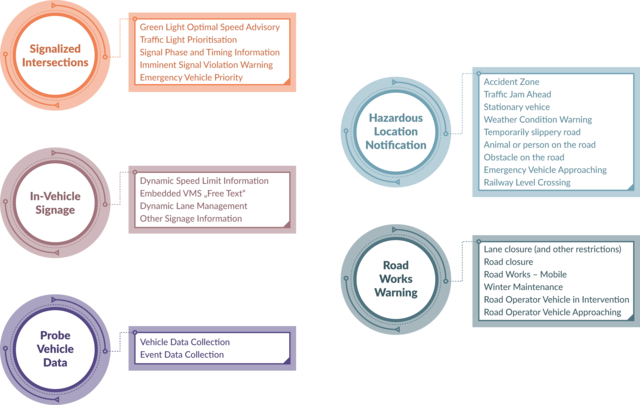
\includegraphics[width=.8\textwidth]{c-its-kolecka.png}
%     \caption{C-ITS use cases \cite{2022}}
%     \label{c-its-use-case}
% \end{figure}

In general, traffic safety and traffic flow improvements can be grouped based on which 
operational tasks they serve \cite{CRoads2021}: 

\begin{itemize}
    \item Provide \emph{information} to road users to improve road safety and comfort.
    \item Display \emph{regulatory boundaries} to inform road users of specific obligations, 
    restrictions or prohibitions
    \item Provide \emph{warnings} to road users about incidents ahead in their exact nature. 
\end{itemize}

% To provide more insight into the design and applications of C-ITS systems, two systems are 
% introduced - In-vehicle Information System and Cooperative Adaptive Cruise Control. These 
% systems were selected because their operation is conditional to user engagement and are 
% considered state-of-the-art applications, utilizing the C-ITS technology specification. For 
% those reasons, they are also relevant to IVS-based research. 

% \subsection{Cooperative Adaptive Cruise Control}

% The Cooperative Adaptive Cruise Control (CACC) is an extension to an already well-proven ITS -
% Adaptive Cruise Control.  As has been described above, this system extends the base (adaptive)
% cruise control system by utilizing the V2V information broadcasted by other road users. The
% system has proved to reduce the number of shock-waves by reducing oscillations that would
% otherwise happen without speed information sharing and increasing capacity of the traffic
% network, albeit only with higher penetration rates ($\ge 40\%$) \cite{van_Arem_2006}. Nonetheless,
% regarding the aspect of driver engagement, the system in itself does not provide any
% extra engagement from the driver side. 

% However, another system called \emph{Green Light Optimization Speed Advisory} (GLOSA), which
% can be considered as an extension of the CACC system utilizes information about signal phasing
% using V2I communication. This system attempts to recommend a speed that would eliminate the
% need to stop before a red light, avoiding idle time. Dedicated A Signal Phase and Timing (SPaT)
% messages are used to coordinate oncoming traffic speed and a Map (MAP) message is to convey
% information about intersection topology. According to \cite{Pariota_2019}, the results of
% simulating the deployment of this system demonstrated that even using a simple control algorithm
% to avoid the stop\&go a reduction of fuel consumption and emissions in the region
% of 5 to 12 \% has been observed. The study in \cite{Katsaros_2011} even concluded that with
% enough penetration, the idle (stop) time could be decreased by more than $70 \%$ (see fig.
% \ref{glosa-chart} below).

% Because of the ongoing research and possibilities of such a system, the proposed simulation architecture 
% should be capable of CACC implementation - facilitating a GLOSA traffic controller simulation deployment
% and respective interface for transmitting such information to vehicles, which will react to a received 
% message, conveying GLOSA timing information accordingly. 

% Should I also delete this ????
% \begin{figure}[htbp]
%     \centering
%     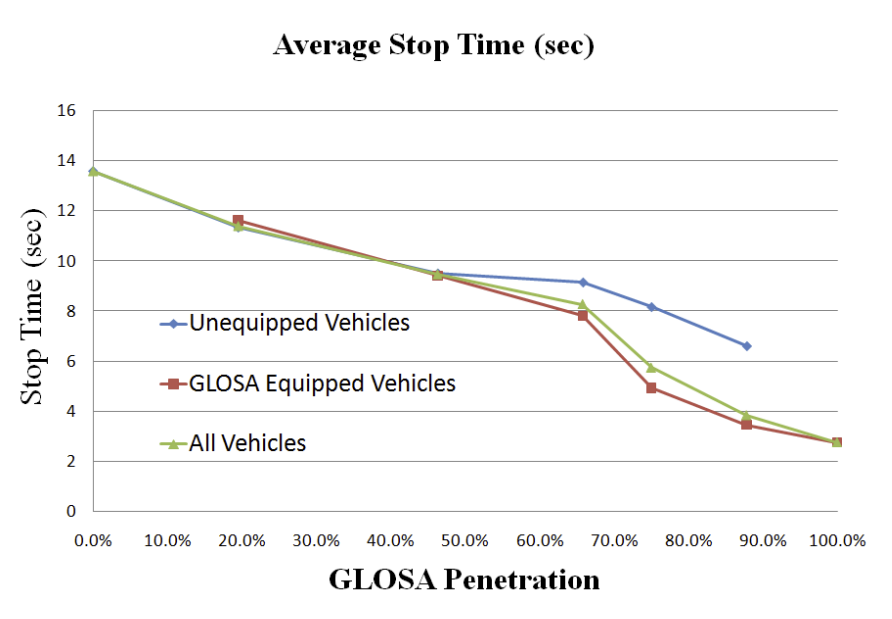
\includegraphics[width=.8\textwidth]{glosa-perf-chart.png} 
%     \caption{Idle time reduction based on GLOSA penetration rate \cite{Katsaros_2011}}
%     \label{glosa-chart}
% \end{figure}

\subparagraph{Project C-Roads}\label{sec-croads}

The C-Roads project was established by the EU member states and road operators to study the
effects and refine the future deployment process of C-ITS.  The project's main objective is to
harmonize C-ITS deployment activities across Europe.  Within the C-Roads project, 6 work groups
(WG) were established, each focusing on a specific topic/scope regarding C-ITS objectives and
priorities for research, testing and pre- deployment of C-ITS \cite{Commision2021}. 

\begin{itemize}
    \itemspacing{0.7}
    \item WG1: Develop an EU agenda for testing
    \item WG2: Coordination and cooperation of R\&I activities
    \item WG3: Physical and digital road infrastructure
    \item WG4: Road Safety
    \item WG5: Access and exchange of data \& cyber-security
    \item WG6: Connectivity and digital infrastructure
\end{itemize}

Regarding the scope of this thesis, \emph{WG3} is the most informative segment because the focus of
this group was, in the first place, regarding the infrastructure support for autonomous
vehicles\footnote{Autonomous vehicles of Level 4 defined by the Society of Automotive
Engineers}. One of the objectives was combining relevant physical and digital infrastructure,
assessing the relevance between them and automated vehicles, and mapping infrastructure
elements to use-cases as \emph{Generic Driving Tasks} (GDTs):

\begin{itemize}
    \item Sensing \& Perception
    \begin{itemize}
        \itemspacing{.7}
        \item Ego localization
        \item Environmental awareness (object classification and incident detection)
        \item Enhanced perception (for limited visibility scenarios)
    \end{itemize}
    \item Planning
    \begin{itemize}
        \itemspacing{.7}
        \item (Dynamic) information and regulations
        \item Safe and appropriate navigation plans
        \item Cooperative planning
    \end{itemize}
    \item Actuation
    \begin{itemize}
        \itemspacing{.7}
        \item Motion Control
        \item Minimum Risk Manoeuvre
    \end{itemize}
\end{itemize}

It is therefore advisable to keep these GDTs Tasks in mind when thinking about the proposed framework 
features. To maximize the number of potential use cases of the designed MAS simulation framework, 
it shall offer basic components to simulate all aforementioned GDTs, as the tasks above will be
a fundamental part of the future C-ITS deployment.

To put these GDT use cases into a better perspective, a mapping was created (table
\ref{gdt-mapping}) that links the aforementioned GDTs to existing, relevant ITS solutions.
This should clear up and simplify the process of defining requirements for the proposed system,
as the new framework requirements could be easily adopted from existing system documentation of
the particular mapped ITS.

\begin{table}[htbp]
    \caption{GDT to ITS mapping}
    \renewcommand{\arraystretch}{1.3}
    \centering\begin{tabular}{lp{7em}lp{10em}} \toprule
        \multicolumn{2}{c}{GDT} & \multicolumn{2}{c}{ITS Mapping}                                                   \\ \cmidrule(r){1-2} \cmidrule(l){3-4}
        Group                   & Name                        & Type       & Description                        \\ \midrule
        \multirow{1}{3cm}
        {Sensing \& Perception} & Ego-localization            & HD Maps    & Geo-fencing                        \\
                                &                             & AD         & Self-driving algorithms            \\
                                & Environmental awareness     & IVIS       & Intersection Collision war.        \\
                                &                             &            & Emergency Vehicle war.             \\
                                &                             &            & Stationary Vehicle war.            \\
                                &                             &            & Traffic Jam war.                   \\
                                &                             &            & Traffic accident war.              \\
                                & Enhanced\newline perception & IVIS       & Overtaking war.                    \\
                                &                             &            & Intersection Collision war.        \\
                                &                             &            & VRU warning                        \\ \midrule
        Planning                & Information and regulations & CACC       & Green Light Optimal Speed Advisory \\
                                & Safe navigation plans       & Navigation & Dynamic Vehicle Routing            \\
                                & Cooperative planning        & AD         & Platooning                         \\ \midrule
        Actuation               & Motion Control              & AD         & Self-driving algorithms            \\
                                & Minimum Risk Manoeuvre      & AD         & Self-driving algorithms            \\ \midrule[1.0pt]
&&&\\
        \textbf{Legend}         &                             &            &                                    \\ \midrule
        Abbreviation            & Meaning                     &            &                                    \\ \midrule% \cmidrule(r){1-2}
        HD                      & \multicolumn{3}{l}
        {High-definition}                                                                                       \\
        AD                      & \multicolumn{3}{l}
        {Autonomous driving}                                                                                    \\
        IVIS                    & \multicolumn{3}{l}
        {In-Vehicle Information Systems}                                                                        \\
        VRU                     & \multicolumn{3}{l}
        {Vulnerable Road User}                                                                                   \\
        CACC                    & \multicolumn{3}{l}
        {Cooperative Adaptive Cruise Control}                                                                   \\ \bottomrule
    \end{tabular}
    \label{gdt-mapping}
\end{table}
\clearpage

\subsection{Conclusion}

In this section, Intelligent Transport Systems are introduced. ITS is an
important part of traffic engineering, utilizing traffic data and mathematical modeling to
reduce congestion, improve traffic safety and reduce emissions. The main focus of this section
is to discuss important features of Intelligent Transport Systems that are related to 
the topic of this thesis. The relationship between the driver and ITS system and intelligence 
distribution across ITS actors is discussed. ITS projects relevant to the thesis topic
are investigated, including the research and developments efforts on the EU level. The results suggested that
C-ITS systems are a hot topic in current research. Furthermore, numerous projects (e.g. C-Roads) have been
built and tested, paving the way for the future of interconnected vehicle mobility. 

\clearpage

\end{document}